% =============================================================================
%  SECTION 1: WHEN MODELS SURPRISE US
%  Emergent Abilities · Chain-of-Thought · Thinking Models
%  30-minute session for executive education
% =============================================================================
\documentclass[aspectratio=169, 12pt, xcolor=dvipsnames]{beamer}

% --- Theme & Appearance -------------------------------------------------------
\usetheme{metropolis}
\setbeamercolor{normal text}{fg=black!85, bg=white}
\setbeamercolor{alerted text}{fg=BrickRed}
\setbeamercolor{frametitle}{bg=black!85, fg=white}
\setbeamertemplate{navigation symbols}{}
\setbeamerfont{title}{size=\Large, series=\bfseries}
\setbeamerfont{frametitle}{size=\large, series=\bfseries}
\setbeamerfont{footnote}{size=\tiny}

% --- Packages -----------------------------------------------------------------
\usepackage[T1]{fontenc}
\usepackage{lmodern}
\usepackage{amsmath, amssymb}
\usepackage{tikz}
\usetikzlibrary{arrows.meta, positioning, decorations.pathreplacing, calc}
\usepackage{pgfplots}
\pgfplotsset{compat=1.18}
\usepackage{booktabs}
\usepackage{appendixnumberbeamer}

% --- Macros -------------------------------------------------------------------
\newcommand{\bigquote}[1]{%
  \begin{center}
    \large\itshape ``#1''
  \end{center}
}
\newcommand{\sourcemark}[1]{\hfill{\tiny\color{gray}#1}}

% --- Metadata -----------------------------------------------------------------
\title{When Models Surprise Us}
\subtitle{Emergent Abilities, Chain-of-Thought, and the Thinking Revolution}
\author{LLM Lab --- Executive Education Program}
\date{2026}
\institute{}

% ==============================================================================
\begin{document}

% --- SLIDE 1: TITLE ----------------------------------------------------------
\begin{frame}[plain]
  \titlepage
  \note{Welcome. In the next 25 minutes we explore two connected phenomena
    that have reshaped AI: the sudden appearance of capabilities at scale,
    and the discovery that making models ``think step by step'' unlocks
    extraordinary reasoning.}
\end{frame}

% --- SLIDE 2: SESSION OVERVIEW ------------------------------------------------
\begin{frame}{The Unifying Thread}

\bigquote{The dynamics of learning in LLMs violate our deepest intuitions.}

\vspace{1em}

\begin{columns}[T]
  \begin{column}{0.48\textwidth}
    \centering
    \textbf{A. Emergent Abilities}\\[0.3em]
    {\small Scale a model 10$\times$ and it\\suddenly writes poetry.\\[0.3em]
    Or is that a measurement artifact?}
  \end{column}
  \begin{column}{0.48\textwidth}
    \centering
    \textbf{B. Chain-of-Thought \&\\Thinking Models}\\[0.3em]
    {\small Ask a model to ``think step by step''\\and it solves competition maths.\\[0.3em]
    Train it with RL and it discovers\\reasoning on its own.}
  \end{column}
\end{columns}

\note{Two stories, one message: we cannot predict when or how AI systems
  will acquire new capabilities, and the methods for unlocking reasoning
  evolved from a simple prompting trick to an entirely new paradigm.}
\end{frame}

% ==============================================================================
%  TOPIC A — EMERGENT ABILITIES
% ==============================================================================

% --- SLIDE 3: THE CAPABILITY LADDER -------------------------------------------
\begin{frame}{What Models Can Do at Each Scale}

\begin{center}
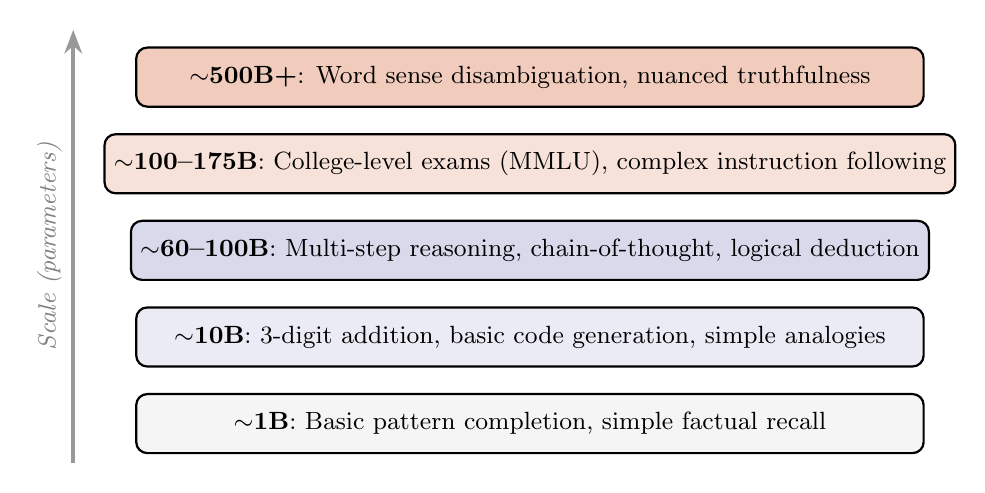
\begin{tikzpicture}[
  font=\small,
  rung/.style={draw, rounded corners, thick, minimum width=10cm,
               minimum height=0.75cm, align=center, fill=#1},
]
  \node[rung=gray!8] (r1) at (0,0) {${\sim}$\textbf{1B}: Basic pattern completion, simple factual recall};
  \node[rung=NavyBlue!8] (r2) at (0,1.1) {${\sim}$\textbf{10B}: 3-digit addition, basic code generation, simple analogies};
  \node[rung=NavyBlue!15] (r3) at (0,2.2) {${\sim}$\textbf{60--100B}: Multi-step reasoning, chain-of-thought, logical deduction};
  \node[rung=BrickRed!10] (r4) at (0,3.3) {${\sim}$\textbf{100--175B}: College-level exams (MMLU), complex instruction following};
  \node[rung=BrickRed!18] (r5) at (0,4.4) {${\sim}$\textbf{500B+}: Word sense disambiguation, nuanced truthfulness};

  \draw[-{Stealth[length=3mm]}, ultra thick, black!40] (-5.8,-0.5) -- (-5.8,5)
    node[midway, left, font=\small\itshape, text=gray, rotate=90, anchor=south] {Scale (parameters)};
\end{tikzpicture}
\end{center}

\vspace{-0.5em}
{\small These are \alert{approximate thresholds} from Wei et al.\ (TMLR 2022).
Capabilities cluster at certain scales rather than appearing uniformly.}
\sourcemark{\cite{wei2022emergent}}

\note{Wei et al.\ examined 8 model families and catalogued 137 emergent abilities.
  The key observation: capabilities don't improve linearly with scale. They
  cluster at certain thresholds, appearing seemingly out of nowhere.}
\end{frame}

% --- SLIDE 4: CONCRETE EXAMPLES -----------------------------------------------
% Speaker note: These examples make emergence concrete. 3-digit addition:
%   0% below 13B, then >80% above. TruthfulQA is especially striking ---
%   medium models are LESS truthful than small ones.
\begin{frame}[fragile]{Concrete Examples: From Nothing to Capability}

\begin{center}
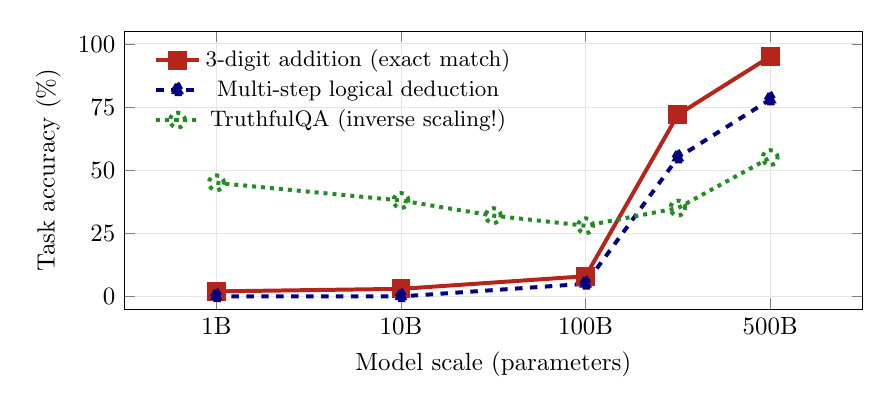
\begin{tikzpicture}[scale=0.9]
  \begin{axis}[
    width=12cm, height=5.5cm,
    xlabel={Model scale (parameters)},
    ylabel={Task accuracy (\%)},
    xmin=0.5, xmax=4.5,
    ymin=-5, ymax=105,
    xtick={1,2,3,4},
    xticklabels={1B, 10B, 100B, 500B},
    ytick={0,25,50,75,100},
    xmajorgrids=true,
    ymajorgrids=true,
    major grid style={gray!20},
    legend pos=north west,
    legend style={font=\small, draw=none, fill=none},
    every axis plot/.append style={ultra thick},
  ]
    \addplot[BrickRed, mark=square*, mark size=3pt] coordinates {
      (1,2) (2,3) (3,8) (3.5,72) (4,95)
    };
    \addlegendentry{3-digit addition (exact match)}
    \addplot[NavyBlue, mark=triangle*, mark size=3pt, dashed] coordinates {
      (1,0) (2,0) (3,5) (3.5,55) (4,78)
    };
    \addlegendentry{Multi-step logical deduction}
    \addplot[ForestGreen, mark=o, mark size=3pt, dotted] coordinates {
      (1,45) (2,38) (2.5,32) (3,28) (3.5,35) (4,55)
    };
    \addlegendentry{TruthfulQA (inverse scaling!)}
  \end{axis}
\end{tikzpicture}
\end{center}

\vspace{-0.5em}
{\small \textbf{3-digit addition}: 0\% $\to$ 80\%+ in a narrow range.
\textbf{TruthfulQA}: medium models are \alert{less truthful} than small ones ---
they've learned misconceptions. Only at 280B+ does truthfulness improve.}
\sourcemark{\cite{wei2022emergent, lin2022truthfulqa}}

\end{frame}

% --- SLIDE 5: MORE IS DIFFERENT -----------------------------------------------
\begin{frame}{``More Is Different'' --- From Physics to AI}

\begin{columns}[c]
  \begin{column}{0.55\textwidth}
    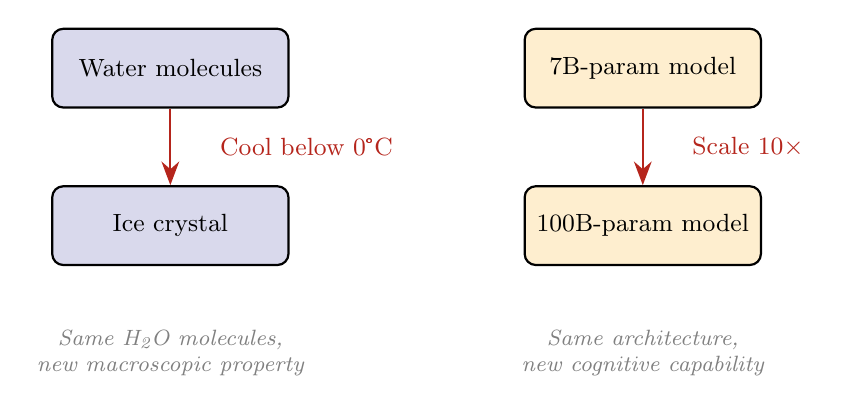
\begin{tikzpicture}[
      every node/.style={font=\small},
      phase/.style={draw, rounded corners, minimum width=3cm,
                    minimum height=1cm, align=center, thick},
    ]
      \node[phase, fill=NavyBlue!15] (water) at (0,0) {Water molecules};
      \node[phase, fill=NavyBlue!15] (ice) at (0,-2) {Ice crystal};
      \draw[-{Stealth[length=3mm]}, thick, BrickRed]
        (water) -- (ice) node[midway, right=5mm]
        {\alert{Cool below 0\textdegree{}C}};

      \node[phase, fill=Dandelion!20] (small) at (6,0) {7B-param model};
      \node[phase, fill=Dandelion!20] (large) at (6,-2) {100B-param model};
      \draw[-{Stealth[length=3mm]}, thick, BrickRed]
        (small) -- (large) node[midway, right=5mm]
        {\alert{Scale 10$\times$}};

      \node[font=\footnotesize\itshape, text=gray, anchor=north,
            align=center] at (0,-3.2)
        {Same H\textsubscript{2}O molecules,\\new macroscopic property};
      \node[font=\footnotesize\itshape, text=gray, anchor=north,
            align=center] at (6,-3.2)
        {Same architecture,\\new cognitive capability};
    \end{tikzpicture}
  \end{column}
  \begin{column}{0.42\textwidth}
    \bigquote{The ability to reduce everything to simple fundamental laws
      does not imply the ability to start from those laws and reconstruct
      the universe.}

    \vspace{0.5em}
    \hfill --- P.W.\ Anderson, 1972 \cite{anderson1972more}

    \vspace{1em}
    {\small Nobel laureate. The same principle that explains why ice
    is rigid may explain why GPT-4 can write code.}
  \end{column}
\end{columns}

\note{Anderson's 1972 essay is the intellectual ancestor of the emergence
  framing. Knowing the fundamental laws of a system does not let you predict
  emergent properties at scale.}
\end{frame}

% --- SLIDE 6: THE MIRAGE REBUTTAL ---------------------------------------------
% Speaker note: Schaeffer et al.\ showed that metric choice can create or
%   destroy the appearance of emergence. The business implication: the truth
%   about what the next model can do is genuinely uncertain.
\begin{frame}[fragile]{Or Is It a Mirage?}

\begin{center}
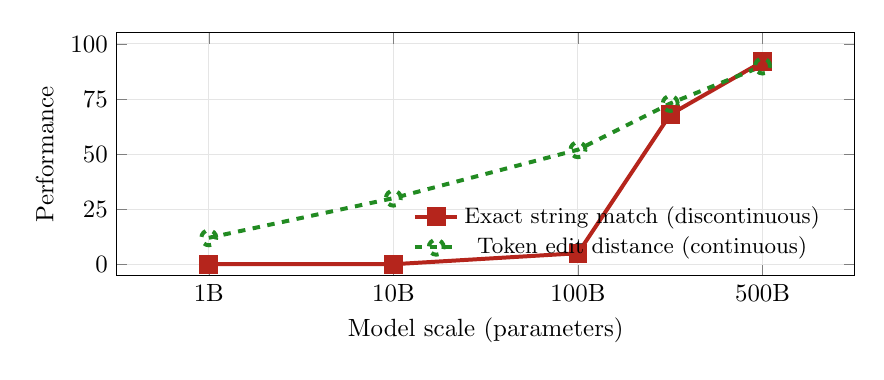
\begin{tikzpicture}[scale=0.9]
  \begin{axis}[
    width=12cm, height=5cm,
    xlabel={Model scale (parameters)},
    ylabel={Performance},
    xmin=0.5, xmax=4.5,
    ymin=-5, ymax=105,
    xtick={1,2,3,4},
    xticklabels={1B, 10B, 100B, 500B},
    ytick={0,25,50,75,100},
    xmajorgrids=true,
    ymajorgrids=true,
    major grid style={gray!20},
    legend pos=south east,
    legend style={font=\small, draw=none, fill=none},
    every axis plot/.append style={ultra thick},
  ]
    \addplot[BrickRed, mark=square*, mark size=3pt] coordinates {
      (1,0) (2,0) (3,5) (3.5,68) (4,92)
    };
    \addlegendentry{Exact string match (discontinuous)}
    \addplot[ForestGreen, mark=o, mark size=3pt, dashed] coordinates {
      (1,12) (2,30) (3,52) (3.5,73) (4,90)
    };
    \addlegendentry{Token edit distance (continuous)}
  \end{axis}
\end{tikzpicture}
\end{center}

\vspace{-0.5em}
\alert{Schaeffer et al.\ (NeurIPS 2023, Outstanding Paper):} 92\% of
claimed emergent abilities in BIG-Bench appeared only under
\textbf{discontinuous metrics} (exact match, multiple-choice grade).
Switch to a continuous metric $\Rightarrow$ smooth, predictable improvement.

\vspace{0.3em}
{\small The resolution: \emph{some} emergence is real, \emph{some} is
measurement artifact. The uncertainty is irreducible.}
\sourcemark{\cite{schaeffer2023mirage}}
\end{frame}

% --- TRANSITION SLIDE A → B --------------------------------------------------
\begin{frame}[standout]
  Capabilities can appear suddenly at scale.\\[1em]
  But what if you could unlock reasoning\\
  \emph{without} scaling the model ---\\[0.5em]
  just by asking it to \alert{think step by step}?
\end{frame}

% ==============================================================================
%  TOPIC B — CHAIN-OF-THOUGHT AND THINKING MODELS
% ==============================================================================

% --- SLIDE 7: THE CoT DISCOVERY -----------------------------------------------
\begin{frame}{Chain-of-Thought: The Discovery That Changed Everything}

\begin{columns}[T]
  \begin{column}{0.48\textwidth}
    \textbf{Standard prompting:}\\[0.3em]
    {\small\texttt{Q: Roger has 5 tennis balls.\\
    He buys 2 cans of 3 balls.\\
    How many does he have?}\\[0.3em]
    \texttt{A: 11}}

    \vspace{1em}
    \textbf{Chain-of-thought:}\\[0.3em]
    {\small\texttt{A: Roger started with 5.\\
    2 cans $\times$ 3 = 6 new balls.\\
    5 + 6 = \alert{11}. The answer is 11.}}
  \end{column}
  \begin{column}{0.48\textwidth}
    \textbf{Key results (PaLM 540B):}

    \vspace{0.5em}
    \begin{tabular}{lc}
      \toprule
      \textbf{Method} & \textbf{GSM8K} \\
      \midrule
      Standard & ${\sim}$18\% \\
      Chain-of-Thought & ${\sim}$\alert{58\%} \\
      \midrule
      Prior SOTA & 55\% \\
      {\scriptsize (fine-tuned + verifier)} & \\
      \bottomrule
    \end{tabular}

    \vspace{0.8em}
    {\small Zero fine-tuning. Just 8 hand-written\\exemplars with reasoning steps.}
    \sourcemark{\cite{wei2022cot}}
  \end{column}
\end{columns}

\note{Wei et al.\ NeurIPS 2022. A pure prompting technique, requiring zero
  training, surpassed a heavily engineered fine-tuned system. The only
  difference: including intermediate reasoning steps in the prompt.}
\end{frame}

% --- SLIDE 8: ZERO-SHOT CoT + SELF-CONSISTENCY --------------------------------
\begin{frame}{Scaling Up: From One Trick to a Toolkit}

\begin{columns}[T]
  \begin{column}{0.48\textwidth}
    \textbf{Zero-shot CoT} {\small (Kojima et al., 2022)}\\[0.5em]

    Just append:\\[0.3em]
    {\large\alert{``Let's think step by step.''}}

    \vspace{0.8em}
    {\small GSM8K: 10.4\% $\to$ \textbf{40.7\%}\\
    MultiArith: 17.7\% $\to$ \textbf{78.7\%}\\[0.5em]
    A single sentence --- no exemplars ---\\
    produces most of the benefit.}
    \sourcemark{\cite{kojima2022zeroshotcot}}
  \end{column}
  \begin{column}{0.48\textwidth}
    \textbf{Self-Consistency} {\small (Wang et al., 2023)}\\[0.5em]

    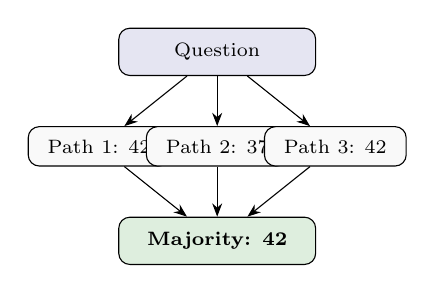
\begin{tikzpicture}[font=\scriptsize, >=Stealth]
      \node[draw, rounded corners, fill=NavyBlue!10, minimum width=2.5cm,
            minimum height=0.6cm] (q) at (0,0) {Question};
      \node[draw, rounded corners, fill=gray!5, minimum width=1.8cm,
            minimum height=0.5cm] (p1) at (-1.5,-1.2) {Path 1: 42};
      \node[draw, rounded corners, fill=gray!5, minimum width=1.8cm,
            minimum height=0.5cm] (p2) at (0,-1.2) {Path 2: 37};
      \node[draw, rounded corners, fill=gray!5, minimum width=1.8cm,
            minimum height=0.5cm] (p3) at (1.5,-1.2) {Path 3: 42};
      \node[draw, rounded corners, fill=ForestGreen!15, minimum width=2.5cm,
            minimum height=0.6cm] (ans) at (0,-2.4) {\textbf{Majority: 42}};
      \draw[->] (q) -- (p1);
      \draw[->] (q) -- (p2);
      \draw[->] (q) -- (p3);
      \draw[->] (p1) -- (ans);
      \draw[->] (p2) -- (ans);
      \draw[->] (p3) -- (ans);
    \end{tikzpicture}

    \vspace{0.5em}
    {\small Sample $N$ reasoning paths,\\majority vote on final answer.\\
    GSM8K: \textbf{+17.9\%} over CoT.\\No extra training needed.}
    \sourcemark{\cite{wang2023selfconsistency}}
  \end{column}
\end{columns}

\note{Kojima showed reasoning is latent. Wang showed that sampling multiple
  paths and voting further improves. Both are pure decoding strategies.}
\end{frame}

% --- SLIDE 9: TREE OF THOUGHTS ------------------------------------------------
\begin{frame}{Tree of Thoughts: Reasoning as Search}

\begin{columns}[c]
  \begin{column}{0.55\textwidth}
    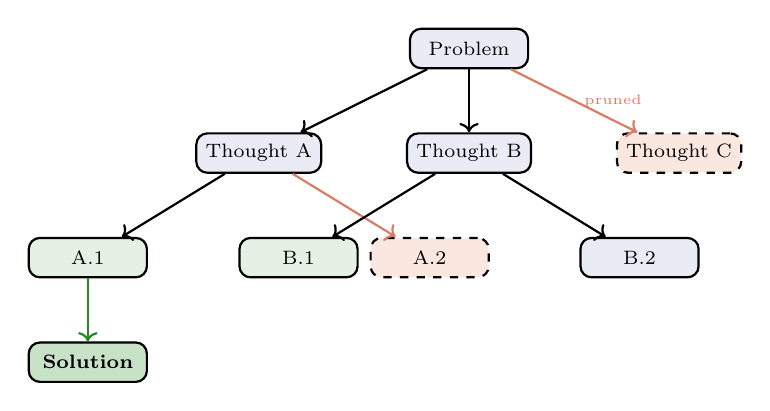
\begin{tikzpicture}[
      font=\scriptsize,
      node distance=0.8cm and 0.6cm,
      tnode/.style={draw, rounded corners, thick, minimum width=1.5cm,
                    minimum height=0.5cm, align=center},
      good/.style={tnode, fill=ForestGreen!12},
      bad/.style={tnode, fill=BrickRed!8, dashed},
      ok/.style={tnode, fill=NavyBlue!8},
    ]
      \node[ok] (root) {Problem};
      \node[ok, below left=of root, xshift=-0.5cm] (a) {Thought A};
      \node[ok, below=of root] (b) {Thought B};
      \node[bad, below right=of root, xshift=0.5cm] (c) {Thought C};

      \node[good, below left=of a] (a1) {A.1};
      \node[bad, below right=of a] (a2) {A.2};
      \node[good, below left=of b] (b1) {B.1};
      \node[ok, below right=of b] (b2) {B.2};

      \node[good, below=of a1, fill=ForestGreen!25] (sol) {\textbf{Solution}};

      \draw[->, thick] (root) -- (a);
      \draw[->, thick] (root) -- (b);
      \draw[->, thick, BrickRed!50] (root) -- (c) node[midway, right, font=\tiny] {pruned};
      \draw[->, thick] (a) -- (a1);
      \draw[->, thick, BrickRed!50] (a) -- (a2);
      \draw[->, thick] (b) -- (b1);
      \draw[->, thick] (b) -- (b2);
      \draw[->, thick, ForestGreen] (a1) -- (sol);
    \end{tikzpicture}
  \end{column}
  \begin{column}{0.42\textwidth}
    \textbf{Yao et al.\ (NeurIPS 2023)}

    \vspace{0.5em}
    {\small Organise reasoning as a \textbf{tree}:
    \begin{enumerate}
      \item Generate multiple thoughts
      \item LLM \emph{evaluates} each
      \item BFS/DFS to explore
      \item Backtrack when stuck
    \end{enumerate}}

    \vspace{0.8em}
    \textbf{Game of 24:}\\
    CoT: \textbf{4\%}\\
    Tree of Thoughts: \alert{\textbf{74\%}}

    \vspace{0.5em}
    {\small 18.5$\times$ improvement from\\organising reasoning as search.}
    \sourcemark{\cite{yao2023tree}}
  \end{column}
\end{columns}

\note{Tree of Thoughts shows that structured search over reasoning is
  dramatically more powerful than a single chain. This is the bridge from
  prompting-based CoT to the thinking model paradigm.}
\end{frame}

% --- SLIDE 10: FROM PROMPTING TO TRAINING -------------------------------------
\begin{frame}{The Leap: From Prompting to Thinking Models}

\begin{center}
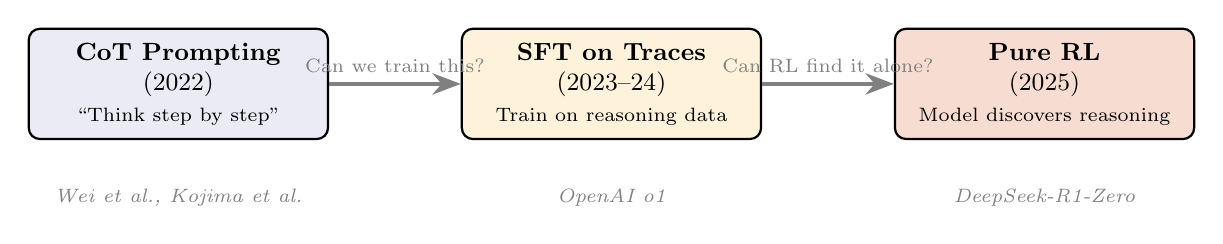
\begin{tikzpicture}[
  font=\small,
  box/.style={draw, rounded corners, thick, minimum width=3.8cm,
              minimum height=1.4cm, align=center},
  >=Stealth,
]
  \node[box, fill=NavyBlue!8] (prompt) at (0,0)
    {\textbf{CoT Prompting}\\(2022)\\{\scriptsize ``Think step by step''}};
  \node[box, fill=Dandelion!15] (sft) at (5.5,0)
    {\textbf{SFT on Traces}\\(2023--24)\\{\scriptsize Train on reasoning data}};
  \node[box, fill=BrickRed!12] (rl) at (11,0)
    {\textbf{Pure RL}\\(2025)\\{\scriptsize Model discovers reasoning}};

  \draw[->, ultra thick, black!50] (prompt) -- (sft)
    node[midway, above, font=\scriptsize] {Can we train this?};
  \draw[->, ultra thick, black!50] (sft) -- (rl)
    node[midway, above, font=\scriptsize] {Can RL find it alone?};

  \node[font=\scriptsize\itshape, text=gray, below=5mm of prompt]
    {Wei et al., Kojima et al.};
  \node[font=\scriptsize\itshape, text=gray, below=5mm of sft]
    {OpenAI o1};
  \node[font=\scriptsize\itshape, text=gray, below=5mm of rl]
    {DeepSeek-R1-Zero};
\end{tikzpicture}
\end{center}

\vspace{0.5em}
{\small The trajectory: a prompting trick (2022) $\to$ trained reasoning models
(2024) $\to$ models that \alert{discover reasoning from scratch via RL} (2025).
This took less than 3 years.}

\note{The conceptual trajectory from prompting to training is the key story.
  CoT showed reasoning is possible, SFT showed it can be trained, and pure RL
  showed it can emerge without human demonstrations.}
\end{frame}

% --- SLIDE 11: THE AHA MOMENT ------------------------------------------------
\begin{frame}{The ``Aha Moment'': Reasoning from Pure Trial and Error}

\begin{center}
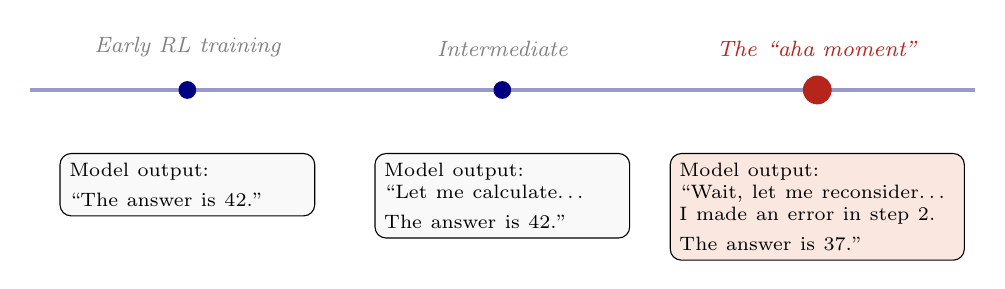
\begin{tikzpicture}[font=\small]
  \draw[ultra thick, NavyBlue!40] (0,0) -- (12,0);

  \node[above, font=\footnotesize\itshape, text=gray] at (2,0.3)
    {Early RL training};
  \node[above, font=\footnotesize\itshape, text=gray] at (6,0.3)
    {Intermediate};
  \node[above, font=\footnotesize\itshape, BrickRed] at (10,0.3)
    {The ``aha moment''};

  \filldraw[NavyBlue] (2,0) circle (3pt);
  \filldraw[NavyBlue] (6,0) circle (3pt);
  \filldraw[BrickRed] (10,0) circle (5pt);

  \node[draw, rounded corners, fill=gray!5, align=left,
        text width=3cm, below=8mm] at (2,0)
    {\scriptsize Model output:\\``The answer is 42.''};

  \node[draw, rounded corners, fill=gray!5, align=left,
        text width=3cm, below=8mm] at (6,0)
    {\scriptsize Model output:\\``Let me calculate\ldots\\The answer is 42.''};

  \node[draw, rounded corners, fill=BrickRed!8, align=left,
        text width=3.5cm, below=8mm] at (10,0)
    {\scriptsize Model output:\\``\alert{Wait, let me reconsider\ldots}\\
     I made an error in step 2.\\The answer is 37.''};
\end{tikzpicture}
\end{center}

\vspace{0.5em}
\textbf{DeepSeek-R1-Zero} (2025): trained with \emph{pure} reinforcement
learning --- no human demonstrations of reasoning.  The model independently
discovered that \alert{pausing to self-correct improves its answers.}
\cite{deepseek2025r1}

\vspace{0.3em}
{\small AIME 2024: 15.6\% $\to$ \textbf{71.0\%} through RL training alone.
With majority voting: \textbf{86.7\%} --- matching OpenAI o1.}

\note{Nobody told the model to think step by step. Through pure trial-and-error
  optimisation, it discovered reflection. The emergent behaviours include
  chain-of-thought, self-verification, and strategy switching.}
\end{frame}

% --- SLIDE 12: BUDGET FORCING -------------------------------------------------
\begin{frame}{Budget Forcing: Controlling How Long a Model Thinks}

\begin{center}
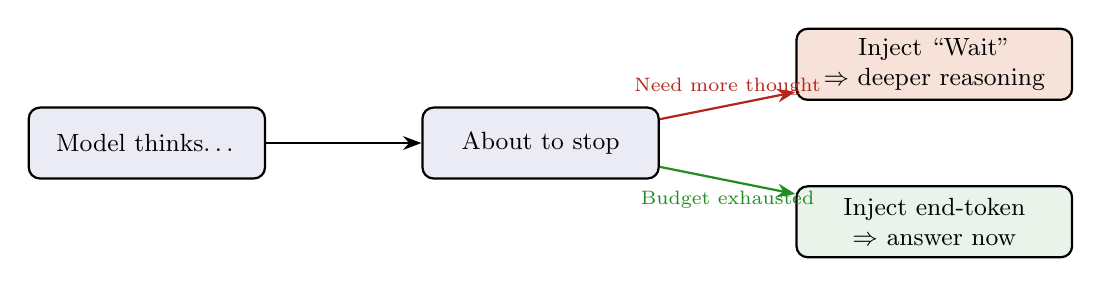
\begin{tikzpicture}[
  font=\small,
  procbox/.style={draw, rounded corners, thick, minimum height=0.9cm,
               align=center, fill=NavyBlue!8},
]
  \node[procbox, minimum width=3cm] (think) at (0,0) {Model thinks\ldots};
  \node[procbox, minimum width=3cm] (stop) at (5,0) {About to stop};

  \node[procbox, fill=BrickRed!10, minimum width=3.5cm] (wait) at (10,1)
    {Inject ``\alert{Wait}''\\$\Rightarrow$ deeper reasoning};

  \node[procbox, fill=ForestGreen!10, minimum width=3.5cm] (force) at (10,-1)
    {Inject end-token\\$\Rightarrow$ answer now};

  \draw[-{Stealth}, thick] (think) -- (stop);
  \draw[-{Stealth}, thick, BrickRed] (stop) -- (wait)
    node[midway, above, font=\scriptsize] {Need more thought};
  \draw[-{Stealth}, thick, ForestGreen] (stop) -- (force)
    node[midway, below, font=\scriptsize] {Budget exhausted};
\end{tikzpicture}
\end{center}

\vspace{0.5em}

\begin{columns}[T]
  \begin{column}{0.50\textwidth}
    \textbf{s1-32B} (Muennighoff et al., 2025):\\
    Fine-tuned on only \textbf{1,000 examples}.\\
    Training: \textbf{26 minutes} on 16 H100s.
    \sourcemark{\cite{muennighoff2025s1}}
  \end{column}
  \begin{column}{0.46\textwidth}
    \begin{tabular}{lc}
      \toprule
      \textbf{Model} & \textbf{AIME 2024} \\
      \midrule
      o1-preview & 44.6\% \\
      s1-32B & 50.0\% \\
      s1-32B + Wait$\times$6 & \alert{57.0\%} \\
      \bottomrule
    \end{tabular}
  \end{column}
\end{columns}

\note{Budget forcing: suppress the stop token and append ``Wait.'' The model
  re-examines its work, often catching errors. 1,000 examples and 26 minutes
  of training beats o1-preview.}
\end{frame}

% --- SLIDE 13: TAXONOMY -------------------------------------------------------
\begin{frame}{The Test-Time Compute Landscape}

\begin{center}
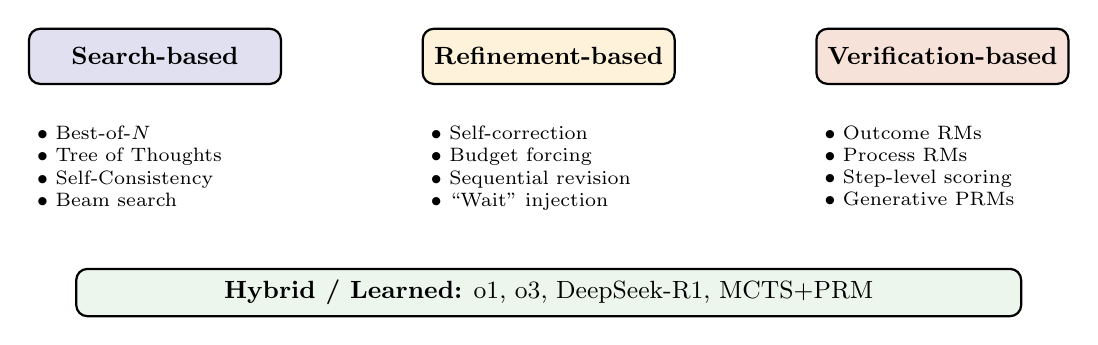
\begin{tikzpicture}[
  font=\small,
  cat/.style={draw, rounded corners, thick, minimum width=3.2cm,
              minimum height=0.7cm, align=center},
  method/.style={font=\scriptsize, align=left, text width=3cm},
]
  % Categories
  \node[cat, fill=NavyBlue!12] (search) at (0,2.5) {\textbf{Search-based}};
  \node[cat, fill=Dandelion!15] (refine) at (5,2.5) {\textbf{Refinement-based}};
  \node[cat, fill=BrickRed!10] (verify) at (10,2.5) {\textbf{Verification-based}};

  % Methods
  \node[method, below=4mm of search] (sm) {
    $\bullet$ Best-of-$N$\\
    $\bullet$ Tree of Thoughts\\
    $\bullet$ Self-Consistency\\
    $\bullet$ Beam search
  };

  \node[method, below=4mm of refine] (rm) {
    $\bullet$ Self-correction\\
    $\bullet$ Budget forcing\\
    $\bullet$ Sequential revision\\
    $\bullet$ ``Wait'' injection
  };

  \node[method, below=4mm of verify] (vm) {
    $\bullet$ Outcome RMs\\
    $\bullet$ Process RMs\\
    $\bullet$ Step-level scoring\\
    $\bullet$ Generative PRMs
  };

  % Hybrid bar at bottom
  \node[draw, rounded corners, thick, fill=ForestGreen!8,
        minimum width=12cm, minimum height=0.6cm, align=center]
    (hybrid) at (5,-0.5)
    {\textbf{Hybrid / Learned:} o1, o3, DeepSeek-R1, MCTS+PRM};
\end{tikzpicture}
\end{center}

\vspace{0.3em}
{\small \textbf{Key insight} (Snell et al., ICLR 2025): A small model with
optimal test-time compute can outperform a \alert{14$\times$ larger model}.
The optimal strategy is prompt-dependent.}
\sourcemark{\cite{snell2025scaling}}

\note{Snell et al.\ showed that compute-optimal test-time allocation yields
  4x efficiency over naive best-of-N. Easy problems favor revision; hard
  problems favor search against a process reward model.}
\end{frame}

% --- SLIDE 14: TWO AXES OF SCALING -------------------------------------------
% Speaker note: The capability frontier has two dimensions. Train-time is
%   capital expense; test-time is per-query operating expense.
\begin{frame}[fragile]{Two Axes of Scaling}

\begin{center}
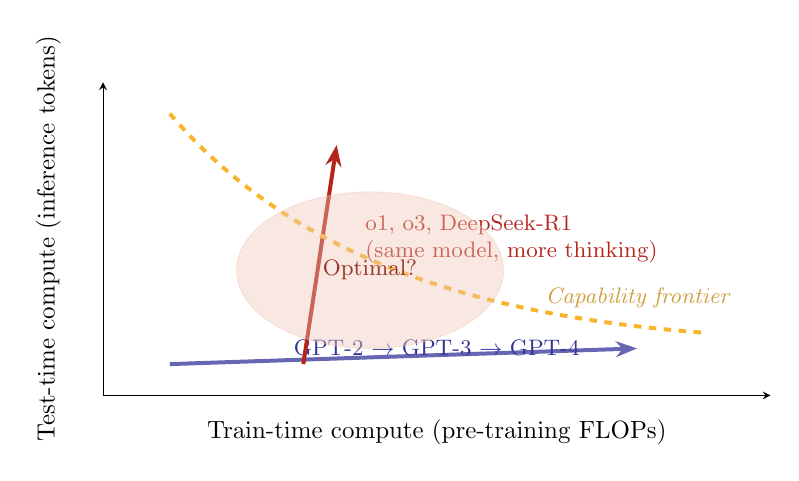
\begin{tikzpicture}[scale=0.9]
  \begin{axis}[
    width=11cm, height=6cm,
    xlabel={Train-time compute (pre-training FLOPs)},
    ylabel={Test-time compute (inference tokens)},
    xmin=0, xmax=10,
    ymin=0, ymax=10,
    xtick=\empty,
    ytick=\empty,
    axis lines=left,
    every axis x label/.style={at={(axis description cs:0.5,-0.05)},
                                anchor=north},
    every axis y label/.style={at={(axis description cs:-0.05,0.5)},
                                anchor=south, rotate=90},
  ]
    \draw[-{Stealth[length=3mm]}, ultra thick, NavyBlue!60]
      (axis cs:1,1) -- (axis cs:8,1.5);
    \node[NavyBlue!80, font=\small, anchor=south] at (axis cs:5,1)
      {GPT-2 $\to$ GPT-3 $\to$ GPT-4};
    \draw[-{Stealth[length=3mm]}, ultra thick, BrickRed]
      (axis cs:3,1) -- (axis cs:3.5,8);
    \node[BrickRed, font=\small, anchor=west, align=left] at (axis cs:3.8,5)
      {o1, o3, DeepSeek-R1\\(same model, more thinking)};
    \draw[ultra thick, Dandelion, dashed]
      (axis cs:1,9) .. controls (axis cs:3,4) and (axis cs:6,2.5)
      .. (axis cs:9,2);
    \node[Dandelion!80!black, font=\small\itshape, anchor=south west]
      at (axis cs:6.5,2.5) {Capability frontier};
    \filldraw[BrickRed!20, opacity=0.4]
      (axis cs:4,4) circle [x radius=2, y radius=2.5];
    \node[font=\small, BrickRed!80!black] at (axis cs:4,4) {Optimal?};
  \end{axis}
\end{tikzpicture}
\end{center}

\vspace{-0.5em}
{\small The capability frontier now has \emph{two dimensions}. The strategic
question for any organisation deploying LLMs: where on this frontier should
you invest?}
\end{frame}

% --- SLIDE 15: DISCUSSION QUESTIONS -------------------------------------------
\begin{frame}{Questions to Take Home}

\begin{enumerate}
  \item[\textbf{1.}] If we cannot predict what the next model will be capable
    of, \alert{how should organisations plan for AI adoption}?\\
    {\small (Emergent abilities mean capability forecasting is unreliable.)}

  \vspace{0.8em}
  \item[\textbf{2.}] Chain-of-thought evolved from a prompting trick to a
    training paradigm in under 3 years.
    \alert{What reasoning capabilities are next}?\\
    {\small (If pure RL can discover self-correction, what else can it discover?)}

  \vspace{0.8em}
  \item[\textbf{3.}] Test-time compute trades latency for accuracy.
    \alert{Which of your business decisions warrant a model that ``thinks
    longer''}?\\
    {\small (Not all queries are equal --- when is 30 seconds of thinking
    worth the cost?)}
\end{enumerate}

\note{Question 1 connects emergence to business strategy. Question 2
  connects CoT evolution to future capabilities. Question 3 connects
  test-time compute to operational decisions.}
\end{frame}

% --- SLIDE 16: CLOSING --------------------------------------------------------
\begin{frame}[standout]
  The dynamics of learning in LLMs\\
  violate our deepest intuitions.\\[1.5em]
  {\normalsize Plan accordingly.}
\end{frame}

% ==============================================================================
%  BIBLIOGRAPHY
% ==============================================================================
\begin{frame}[allowframebreaks]{References}
  \footnotesize
  \begin{thebibliography}{99}

    \bibitem{anderson1972more}
    P.W.\ Anderson.
    \newblock More Is Different.
    \newblock \emph{Science}, 177(4047):393--396, 1972.

    \bibitem{wei2022emergent}
    J.\ Wei, Y.\ Tay, R.\ Bommasani, C.\ Raffel, B.\ Zoph, S.\ Borgeaud
    et al.
    \newblock Emergent Abilities of Large Language Models.
    \newblock \emph{Transactions on Machine Learning Research (TMLR)}, 2022.

    \bibitem{lin2022truthfulqa}
    S.\ Lin, J.\ Hilton, O.\ Evans.
    \newblock TruthfulQA: Measuring How Models Mimic Human Falsehoods.
    \newblock \emph{ACL}, 2022.

    \bibitem{schaeffer2023mirage}
    R.\ Schaeffer, B.\ Miranda, S.\ Koyejo.
    \newblock Are Emergent Abilities of Large Language Models a Mirage?
    \newblock \emph{NeurIPS}, 2023. \textbf{Outstanding Paper Award.}

    \bibitem{wei2022cot}
    J.\ Wei, X.\ Wang, D.\ Schuurmans, M.\ Bosma, B.\ Ichter, F.\ Xia,
    E.\ Chi, Q.V.\ Le, D.\ Zhou.
    \newblock Chain-of-Thought Prompting Elicits Reasoning in Large Language
    Models.
    \newblock \emph{NeurIPS}, 2022.

    \bibitem{kojima2022zeroshotcot}
    T.\ Kojima, S.S.\ Gu, M.\ Reid, Y.\ Matsuo, Y.\ Iwasawa.
    \newblock Large Language Models are Zero-Shot Reasoners.
    \newblock \emph{NeurIPS}, 2022.

    \bibitem{wang2023selfconsistency}
    X.\ Wang, J.\ Wei, D.\ Schuurmans, Q.V.\ Le, E.\ Chi et al.
    \newblock Self-Consistency Improves Chain of Thought Reasoning in Language
    Models.
    \newblock \emph{ICLR}, 2023.

    \bibitem{yao2023tree}
    S.\ Yao, D.\ Yu, J.\ Zhao, I.\ Shafran, T.L.\ Griffiths, Y.\ Cao,
    K.\ Narasimhan.
    \newblock Tree of Thoughts: Deliberate Problem Solving with Large Language
    Models.
    \newblock \emph{NeurIPS}, 2023.

    \bibitem{deepseek2025r1}
    DeepSeek-AI, D.\ Guo, D.\ Yang et al.
    \newblock DeepSeek-R1: Incentivizing Reasoning Capability in LLMs via
    Reinforcement Learning.
    \newblock \emph{arXiv:2501.12948}, 2025. Published in \emph{Nature}.

    \bibitem{muennighoff2025s1}
    N.\ Muennighoff, Z.\ Yang, W.\ Shi, X.L.\ Li, L.\ Fei-Fei et al.
    \newblock s1: Simple Test-Time Scaling.
    \newblock \emph{arXiv:2501.19393}, 2025.

    \bibitem{snell2025scaling}
    C.\ Snell, J.\ Lee, K.\ Xu, A.\ Kumar.
    \newblock Scaling LLM Test-Time Compute Optimally Can Be More Effective
    Than Scaling Model Parameters.
    \newblock \emph{ICLR}, 2025. Oral.

  \end{thebibliography}
\end{frame}

\end{document}
